\documentclass[a4paper,xelatex,10pt,ja=standard,twocolumn]{bxjsarticle}

%% \XeLaTeXロゴ
\usepackage{metalogo}
%% subfigureのモダンな書き方のため
\usepackage[hang,small,bf]{caption}
\usepackage[subrefformat=parens]{subcaption}
\renewcommand{\subfigureautorefname}{\figureautorefname}
%% 箇条書き
\usepackage{enumerate}
%% bib
\usepackage[square,comma,numbers,sort&compress]{natbib}
%% ソースコードを貼り付けるため
\usepackage{listings, color}
%% 必須っぽい
\usepackage{amsmath, amssymb}
%% レイアウトのため
\usepackage{geometry, layout}
\geometry{top=2cm, bottom=2cm, left=1.5cm, right=1.5cm, includefoot}
%% リンクを貼るため
%% \usepackage[pdfborder={0 0 0}]{hyperref}
\usepackage[pdfborder={0 0 0}, colorlinks=true, pdfencoding=auto]{hyperref}
\newcommand*{\fullref}[1]{\hyperref[{#1}]{\autoref*{#1} \nameref*{#1}}}
\hypersetup{bookmarks=true,
        bookmarksnumbered=true,
        hidelinks,
        setpagesize=false,
        pdfauthor={EisokuKuroiwa}}

\author{Eisoku Kuroiwa}

\hypersetup{pdftitle={KalmanFilter},
        pdfsubject={memo},
        pdfkeywords={kf, ekf}}
\usepackage{setspace}
\title{姿勢推定のためのKalmanFilter}

\begin{document}
\maketitle

目次

\begin{itemize}
  \item \fullref{sec:knowledge_about_rotation}
  \item \fullref{sec:rpy_kalman_filter}
  \item \fullref{sec:quaternion_kalman_filter}
\end{itemize}

\section{回転に関する知識} \label{sec:knowledge_about_rotation}

ここでは姿勢推定のKalmanFilterを意識しつつ,
回転に関するもろもろの知識をまとめて,証明する.

証明することは

\begin{description}
\item[\fullref{subsec:gyro}]\mbox{}\\
  ある剛体$A$が回転している時に,その剛体の角速度ベクトルをworld座標系$W$で表記した$\boldsymbol{\omega}^{W}$とworld座標系$W$相対の$A$の回転行列${}^{W}_{A}\boldsymbol{R}$の間には
  \begin{equation}
    {}^{W}_{A}\dot{\boldsymbol{R}} {}^{W}_{A}\boldsymbol{R}^{T} =
    {\scriptstyle
      \begin{pmatrix}
        0  & -\omega^{W}_{z} & \omega^{W}_{y}\\
        \omega^{W}_{z} & 0 & -\omega^{W}_{x}\\
        - \omega^{W}_{y}  & \omega^{W}_{x} & 0
    \end{pmatrix}}
    = [\boldsymbol{\omega}^{W}]_{\times}
  \end{equation}
  が成り立つ.
  ここでいう$\boldsymbol{\omega}^{W}$はworld座標系の角速度ベクトルであって,
  IMUが出力するようなlocal座標系の角速度ベクトルではないことが重要.
\item[\fullref{subsec:rpy}]\mbox{}\\
  剛体$A$の角速度ベクトルを$A$座標系相対で表記した$\boldsymbol{\omega}^{A}$がIMUから取得できる.
  それと,world座標系$W$相対の$A$の回転行列${}^{W}_{A}\boldsymbol{R}$をロール・ピッチ・ヨーに変換したものの関係式は
  \begin{equation}
    \begin{pmatrix}
      \dot{\alpha} \\
      \dot{\beta} \\
      \dot{\gamma}
    \end{pmatrix} =
    \begin{pmatrix}
      1 & \frac{\sin \alpha \sin \beta}{\cos \beta} & \frac{\cos \alpha \sin \beta}{\cos \beta} \\
      0 & \cos \alpha & - \sin \alpha \\
      0 & \frac{\sin \alpha}{\cos \beta} & \frac{\cos \alpha}{\cos \beta}
    \end{pmatrix}
    \begin{pmatrix}
      \boldsymbol{\omega}^{A}_{x}\\
      \boldsymbol{\omega}^{A}_{y}\\
      \boldsymbol{\omega}^{A}_{z}
    \end{pmatrix}
  \end{equation}
  である.
\item[\fullref{subsec:quat}]\mbox{}\\
  同様に,クォータニオン$\tilde{\boldsymbol{q}}$を使って表記すると
  \begin{align}
    \dot{\tilde{\boldsymbol{q}}} & = \frac{1}{2}\boldsymbol{\omega}^{W}\tilde{\boldsymbol{q}}\\
    & = \frac{1}{2}\tilde{\boldsymbol{q}}\boldsymbol{\omega}^{A}\\
    & = \frac{1}{2}
    \begin{pmatrix}
      0                           & - \boldsymbol{\omega}^{A}_{x} & - \boldsymbol{\omega}^{A}_{y} & - \boldsymbol{\omega}^{A}_{z}\\
      \boldsymbol{\omega}^{A}_{x} & 0                             &   \boldsymbol{\omega}^{A}_{z} & - \boldsymbol{\omega}^{A}_{y}\\
      \boldsymbol{\omega}^{A}_{y} & - \boldsymbol{\omega}^{A}_{z} & 0                             &   \boldsymbol{\omega}^{A}_{x}\\
      \boldsymbol{\omega}^{A}_{z} &   \boldsymbol{\omega}^{A}_{y} & - \boldsymbol{\omega}^{A}_{x} & 0
    \end{pmatrix}
    \tilde{\boldsymbol{q}}
  \end{align}
  となる.
  ただし,スカラー部を$q_0$,ベクトル部を$\boldsymbol{q} = (q_1, q_2, q_3)$として,
  $\tilde{\boldsymbol{q}} = (q_0, \boldsymbol{q})$とした.
\item[\fullref{subsec:acc}]\mbox{}\\
  \url{http://knock.t.u-tokyo.ac.jp/lecture/pdf_data01/5.pdf}の式(14)に詳しいが,
  \begin{equation}
    \boldsymbol{a}^{A} = \dot{\boldsymbol{v}}^{A} + \boldsymbol{\omega}^{A} \times \boldsymbol{v}^{A} + {}^{W}_{A}\boldsymbol{R}^{T}
    \begin{pmatrix}
      0\\
      0\\
      +g
    \end{pmatrix}
  \end{equation}
  いや,これは微妙かも.違うかもしれない.難しいので,一旦置いておく.
\item[\fullref{subsec:quat-dcm}]\mbox{}\\
  \begin{equation}
    {}^{W}_{A}\boldsymbol{R} =
    {\tiny
      \begin{pmatrix}
        q_0^2+q_1^2-q_2^2-q_3^2 & 2\left(q_1 q_2 + q_0 q_3\right) & 2\left(q_1 q_3 - q_0 q_2\right)\\
        2\left(q_1 q_2 - q_0 q_3\right) & q_0^2-q_1^2+q_2^2-q_3^2 & 2\left(q_2 q_3 - q_0 q_1\right)\\
        2\left(q_1 q_3 - q_0 q_2\right) & 2\left(q_2 q_3 - q_0 q_1\right) & q_0^2-q_1^2-q_2^2+q_3^2
      \end{pmatrix}
    }
  \end{equation}
\end{description}

である.

\subsection{回転行列の角速度の関係}\label{subsec:gyro}

\subsubsection{証明}
${}^{W}_{A}\boldsymbol{R}$は回転行列なので,
\begin{equation}
  {}^{W}_{A}\boldsymbol{R} {}^{W}_{A}\boldsymbol{R}^{T} = \boldsymbol{E}
\end{equation}
が成り立つ.
この両辺を微分すると
\begin{align}
  & \frac{d}{dt}\{{}^{W}_{A}\boldsymbol{R} {}^{W}_{A}\boldsymbol{R}^{T}\} = \frac{d}{dt}\boldsymbol{E}\\
  \Leftrightarrow & {}^{W}_{A}\dot{\boldsymbol{R}} {}^{W}_{A}\boldsymbol{R}^{T} + {}^{W}_{A}\boldsymbol{R} {}^{W}_{A}\dot{\boldsymbol{R}}^{T} = \boldsymbol{O}\\
  \Leftrightarrow & {}^{W}_{A}\dot{\boldsymbol{R}} {}^{W}_{A}\boldsymbol{R}^{T} + \{{}^{W}_{A}\dot{\boldsymbol{R}} {}^{W}_{A}\boldsymbol{R}^{T}\}^{T} = \boldsymbol{O}
\end{align}
となるので,${}^{W}_{A}\dot{\boldsymbol{R}} {}^{W}_{A}\boldsymbol{R}^{T}$は歪対称行列だと分かる.
よって
\begin{align}
  & {}^{W}_{A}\dot{\boldsymbol{R}} {}^{W}_{A}\boldsymbol{R}^{T} =
  \begin{pmatrix}
    0 & -c & b\\
    c &  0 & -a\\
    b &  a & 0\\
  \end{pmatrix}\\
  \Leftrightarrow & {}^{W}_{A}\dot{\boldsymbol{R}} {}^{W}_{A}\boldsymbol{R}^{T} = [X]_{\times}\\
  \Leftrightarrow & {}^{W}_{A}\dot{\boldsymbol{R}} = [X]_{\times} {}^{W}_{A}\boldsymbol{R} \label{eq:proposal}
\end{align}
となる$X$が存在する.
ここで,$A$の原点から伸びているとあるベクトル$\boldsymbol{p}^{A}$を考える.
$\boldsymbol{p}^{A}$は$A$に固定されていて,一緒に動く.
\autoref{eq:proposal}を利用すると
\begin{align}
  & {}^{W}_{A}\dot{\boldsymbol{R}} \boldsymbol{p}^{A} = [X]_{\times} {}^{W}_{A}\boldsymbol{R} \boldsymbol{p}^{A}\\
  \Leftrightarrow & {}^{W}_{A(t)}\dot{\boldsymbol{R}} \boldsymbol{p}^{A(t)} = [X]_{\times} {}^{W}_{A(t)}\boldsymbol{R} \boldsymbol{p}^{A(t)}\\
  \Leftrightarrow & {}^{W}_{A}\dot{\boldsymbol{R}} \boldsymbol{p}^{A} = [X]_{\times} \boldsymbol{p}^{W}_{t}\\
  \Leftrightarrow & \lim_{\Delta t \to 0} \frac{{}^{W}_{A}\boldsymbol{R}(t+ \Delta t) - {}^{W}_{A}\boldsymbol{R}(t)}{\Delta t} \boldsymbol{p}^{A} = [X]_{\times} \boldsymbol{p}^{W}\\
  \Leftrightarrow & \lim_{\Delta t \to 0} \frac{\boldsymbol{p}^{W}_{t+ \Delta t} - \boldsymbol{p}^{W}_{t}}{\Delta t} = [X]_{\times} \boldsymbol{p}^{W} \label{eq:bibun}
\end{align}
となる.
$\boldsymbol{p}^{W}_{t}$は時刻$t$のときの座標系$W$で表記したベクトルとなる.
$\boldsymbol{p}^{W}_{t+ \Delta t}$は$\boldsymbol{p}^{W}_{t}$を
とあるベクトル$\boldsymbol{s}^{W}$周りに微少量$\Delta \theta$だけ回転させたものと考えられて,
\begin{equation}
  \boldsymbol{p}^{W}_{t+ \Delta t} = \boldsymbol{p}^{W}_{t} + \Delta \boldsymbol{p}
\end{equation}
と表現すると
\begin{gather}
  \Delta \boldsymbol{p}\text{の向き} = \boldsymbol{s}^{W} \times \boldsymbol{p}^{W}_{t}\text{の向き}\\
  \Delta \boldsymbol{p}\text{の大きさ} = \lVert \boldsymbol{p}^{W}_{t} \rVert \Delta \theta
\end{gather}
つまり
\begin{align}
  \Delta \boldsymbol{p} &= \frac{\boldsymbol{s}^{W} \times \boldsymbol{p}^{W}_t}{\lVert \boldsymbol{s}^{W} \times \boldsymbol{p}^{W}_t \rVert} \lVert \boldsymbol{p}^{W}_t \rVert \Delta \theta\\
  & = \frac{\boldsymbol{s}^{W} \times \boldsymbol{p}^{W}_t}{\lVert \boldsymbol{s}^{W} \rVert \lVert \boldsymbol{p}^{W}_t \rVert \sin \left(\frac{\pi}{2}\right)} \lVert \boldsymbol{p}^{W}_t \rVert \Delta \theta\\
  & = \frac{\boldsymbol{s}^{W}}{\lVert \boldsymbol{s}^{W} \rVert} \times \boldsymbol{p}^{W}_t\Delta \theta
\end{align}
なので,\autoref{eq:bibun}より
\begin{align}
  & \lim_{\Delta t \to 0} \frac{\boldsymbol{p}^{W}_{t+ \Delta t} - \boldsymbol{p}^{W}_{t}}{\Delta t} = [X]_{\times} \boldsymbol{p}^{W}\\
  \Leftrightarrow & \lim_{\Delta t \to 0} \frac{\frac{\boldsymbol{s}^{W}}{\lVert \boldsymbol{s}^{W} \rVert} \times \boldsymbol{p}^{W}_{t}\Delta \theta}{\Delta t} = [X]_{\times} \boldsymbol{p}^{W}\\
  \Leftrightarrow & \lim_{\Delta t \to 0} \frac{\boldsymbol{s}^{W}}{\lVert \boldsymbol{s}^{W} \rVert} \frac{\Delta \theta}{\Delta t} \times \boldsymbol{p}^{W} = [X]_{\times} \boldsymbol{p}^{W}\\
  \Leftrightarrow & \boldsymbol{\omega}^{W} \times \boldsymbol{p}^{W} = [X]_{\times} \boldsymbol{p}^{W}\label{eq:result}
\end{align}
となる.
よって,$[X]_{\times} = [\boldsymbol{\omega}^{W}]_{\times}$と分かった.

\autoref{eq:proposal}より,
\begin{equation}
  {}^{W}_{A}\dot{\boldsymbol{R}} = [\boldsymbol{\omega}^{W}]_{\times} {}^{W}_{A}\boldsymbol{R}
\end{equation}
となって証明できた.

ここでいう$\boldsymbol{\omega}^{W}$はworld座標系の角速度ベクトルであって,
IMUが出力するようなlocal座標系の角速度ベクトルではないことが重要.

\subsubsection{具体例で実験}\label{subsubsec:test1}
\autoref{fig:example}のようなパターンを考える.
\begin{figure}[ht]
  \centering
  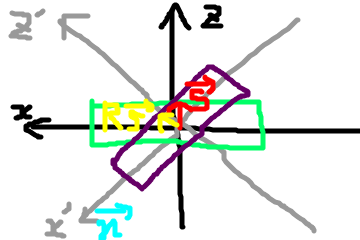
\includegraphics[width=0.8\columnwidth]{figs/section1/example}
  \caption{黒い座標を$W$の座標系,BODYリンクを想定した直方体がworld座標系の原点に最初あって(緑色の直方体),今はピッチ軸周りに45度回転して(灰色座標および紫色の直方体)いる状態.ここからさらに水色の軸$\boldsymbol{n}$周りに$\Delta \eta$回転しようとしている.はてなブログから持ってきたのであれだけど,黄色のベクトルが$\boldsymbol{p}^{A}$}
  \label{fig:example}
\end{figure}
このとき,
\begin{gather}
  {}^{W}_{A(t)}\boldsymbol{R} = \begin{pmatrix}
    \frac{1}{\sqrt{2}} & 0 & \frac{1}{\sqrt{2}}\\
    0 & 1 & 0\\
    -\frac{1}{\sqrt{2}} & 0 & \frac{1}{\sqrt{2}}
  \end{pmatrix}\\
  {}^{A(t)}_{A(t+\Delta t)}\boldsymbol{R} = \begin{pmatrix}
    1 & 0 & 0\\
    0 & \cos \Delta \eta & - \sin \Delta \eta\\
    0 & \sin \Delta \eta &   \cos \Delta \eta
  \end{pmatrix}\\
  \boldsymbol{p}^{A} = \begin{pmatrix}
    0\\
    0\\
    1
  \end{pmatrix}
\end{gather}
となる.
回転行列は\autoref{listing:matirx_from_euler}で求められる.

\lstinputlisting[language=Python, caption=matrix\_from\_euler.py, label=listing:matirx_from_euler, numbers=left, showstringspaces=false,
  keywordstyle={\bfseries \color[cmyk]{1,0,0.1,0}},
  stringstyle={\ttfamily \color[cmyk]{0.5,0,1,0}},
  basicstyle=\ttfamily\small]{codes/matrix_from_euler.py}

\autoref{eq:bibun}の左辺は
\begin{gather}
  \begin{align}
    \boldsymbol{p}^{W}_{t+ \Delta t} &= {}^{W}_{A(t+ \Delta t)}\boldsymbol{R}\boldsymbol{p}^{A}\\
    &= {}^{W}_{A(t)}\boldsymbol{R}{}^{A(t)}_{A(t+ \Delta t)}\boldsymbol{R}\boldsymbol{p}^{A}\\
    &= \begin{pmatrix}
      \frac{\cos \Delta \eta}{\sqrt{2}}\\
      - \sin \Delta \eta\\
      \frac{\cos \Delta \eta}{\sqrt{2}}
    \end{pmatrix}\\
    &\simeq \begin{pmatrix}
      \frac{1}{\sqrt{2}}\\
      - \Delta \eta\\
      \frac{1}{\sqrt{2}}
    \end{pmatrix}
  \end{align}\\
  \boldsymbol{p}^{W}_{t} = \begin{pmatrix}
    \frac{1}{\sqrt{2}}\\
    0\\
    \frac{1}{\sqrt{2}}
  \end{pmatrix}
\end{gather}
より,
\begin{align}
  \lim_{\Delta t \to 0} \frac{\boldsymbol{p}^{W}_{t+ \Delta t} - \boldsymbol{p}^{W}_{t}}{\Delta t} &= \begin{pmatrix}
    0\\
    -\frac{\Delta \eta}{\Delta t}\\
    0
  \end{pmatrix}
\end{align}\\
\autoref{eq:bibun}と\autoref{eq:result}から,$\boldsymbol{\omega}^{W}$は
\begin{equation}
  \boldsymbol{\omega}^{W} \times \begin{pmatrix}
    \frac{1}{\sqrt{2}}\\
    0\\
    \frac{1}{\sqrt{2}}
  \end{pmatrix} = \begin{pmatrix}
    0\\
    -\frac{\Delta \eta}{\Delta t}\\
    0
  \end{pmatrix}\label{eq:target}
\end{equation}
を満たすはず.
\begin{equation}
  \boldsymbol{\omega}^{A} = \begin{pmatrix}
    \frac{\Delta \eta}{\Delta t}\\
    0\\
    0
  \end{pmatrix}
\end{equation}
なので,
\begin{equation}
  \boldsymbol{\omega}^{W} = {}^{W}_{A(t)}\boldsymbol{R} \boldsymbol{\omega}^{A} = \begin{pmatrix}
    \frac{1}{\sqrt{2}} \frac{\Delta \eta}{\Delta t}\\
    0\\
    -\frac{1}{\sqrt{2}} \frac{\Delta \eta}{\Delta t}
  \end{pmatrix}
\end{equation}
であるが,これは\autoref{eq:target}を満たすので,合っている.

ジャイロセンサが感知するのは,$\boldsymbol{\omega}^{A}$の方.

\subsection{回転行列とRPYの関係}\label{subsec:rpy}
\subsubsection{証明}
\url{https://www.jstage.jst.go.jp/article/sicetr1965/40/11/40_11_1160/_pdf}が参考になるし,このテクニックはすごい気がする.

RPYは,オイラー角の一種で,Z$\to$Y$\to$Xの順番で軸周りに回転していくスタイル.
回転角度を順に,Yaw($\gamma$)$\to$Pitch($\beta$)$\to$Roll($\alpha$)と呼ぶ.
これを使って回転行列を表現すると
\begin{equation}
  \boldsymbol{R} = {\tiny \begin{pmatrix}
      \cos \beta \cos \gamma & \sin \alpha \sin \beta \cos \gamma - \cos \alpha \sin \gamma & \cos \alpha \sin \beta \cos \gamma + \sin \alpha \sin \gamma \\
      \cos \beta \sin \gamma & \sin \alpha \sin \beta \sin \gamma + \cos \alpha \cos \gamma & \cos \alpha \sin \beta \sin \gamma - \sin \alpha \cos \gamma \\
      -\sin \beta & \sin \alpha \cos \beta & \cos \alpha \cos \beta
  \end{pmatrix}}\label{eq:DCM}
\end{equation}
となる.

一方,$[\boldsymbol{\omega}]_{\times} = \dot{\boldsymbol{R}} \boldsymbol{R}^{T}$であり,
\begin{align}
  [\boldsymbol{\omega}]_{\times} &=
  \begin{pmatrix}
    0  & -\omega_{z} & \omega_{y}\\
    \omega_{z} & 0 & -\omega_{x}\\
    - \omega_{y}  & \omega_{x} & 0
  \end{pmatrix}\\
  &= \omega_{x} \boldsymbol{X}_1 + \omega_{y} \boldsymbol{X}_2 + \omega_{z} \boldsymbol{X}_3\\
  \boldsymbol{X}_1 &=
  \begin{pmatrix}
    0 & 0 & 0\\
    0 & 0 & -1\\
    0 & 1 & 0
  \end{pmatrix}\\
  \boldsymbol{X}_2 &=
  \begin{pmatrix}
    0 & 0 & 1\\
    0 & 0 & 0\\
    1 & 0 & 0
  \end{pmatrix}\\
  \boldsymbol{X}_3 &=
  \begin{pmatrix}
    0 & -1 & 0\\
    1 & 0 & 0\\
    0 & 0 & 0
  \end{pmatrix}
\end{align}
となって,ここで急に
\begin{gather}
  \boldsymbol{X}_1 \boldsymbol{X}_1 \boldsymbol{X}_1^{T} = \boldsymbol{X}_1\\
  \boldsymbol{X}_1 \boldsymbol{X}_2 \boldsymbol{X}_1^{T} = \boldsymbol{O}\\
  \boldsymbol{X}_1 \boldsymbol{X}_3 \boldsymbol{X}_1^{T} = \boldsymbol{O}
\end{gather}
という関係式を思いつくことができれば,
\begin{gather}
  \omega_{x} \boldsymbol{X}_1 = \boldsymbol{X}_1 [\boldsymbol{\omega}]_{\times} \boldsymbol{X}_1^{T}\\
  \omega_{y} \boldsymbol{X}_2 = \boldsymbol{X}_2 [\boldsymbol{\omega}]_{\times} \boldsymbol{X}_2^{T}\\
  \omega_{z} \boldsymbol{X}_3 = \boldsymbol{X}_3 [\boldsymbol{\omega}]_{\times} \boldsymbol{X}_3^{T}
\end{gather}
という境地に達する.
これを使うと,割と簡単に$[\boldsymbol{\omega}]_{\times} = \dot{\boldsymbol{R}} \boldsymbol{R}^{T}$をオイラー角の微分について整理することが可能になる.(この境地に達しないと,回転行列の微分をして,,,のようにゴリゴリ計算しないといけなくて,sympyを使ってもちょっと無理だった.)

どう簡単になるかというと,りあえず最初の式に注目すると,
\begin{align}
  & \omega_{x} \boldsymbol{X}_1 = \boldsymbol{X}_1 [\boldsymbol{\omega}]_{\times} \boldsymbol{X}_1^{T}\\
  \Leftrightarrow & \omega_{x} \boldsymbol{X}_1 = \boldsymbol{X}_1 \dot{\boldsymbol{R}} \boldsymbol{R}^{T} \boldsymbol{X}_1^{T}\\
  \Leftrightarrow & \omega_{x} \boldsymbol{X}_1 = \left(\boldsymbol{X}_1 \dot{\boldsymbol{R}}\right) \left(\boldsymbol{X}_1 \boldsymbol{R}\right)^{T}
\end{align}
が成り立つ.
\begin{equation}
  \boldsymbol{R} = \begin{pmatrix}
      a_{11} & a_{12} & a_{13}\\
      a_{21} & a_{22} & a_{23}\\
      a_{31} & a_{32} & a_{33}
  \end{pmatrix}
\end{equation}
と置くと,
\begin{align}
  & \omega_{x} \boldsymbol{X}_1 = \left(\boldsymbol{X}_1 \dot{\boldsymbol{R}}\right) \left(\boldsymbol{X}_1 \boldsymbol{R}\right)^{T}\\
  \Leftrightarrow & \omega_{x} \boldsymbol{X}_1 =
  \begin{pmatrix}
    0 & 0 & 0\\
    - \dot{a}_{31} & - \dot{a}_{32} & - \dot{a}_{33}\\
    \dot{a}_{21} & \dot{a}_{22} & \dot{a}_{23}
  \end{pmatrix}
  \begin{pmatrix}
    0 & - a_{31} & a_{21}\\
    0 & - a_{32} & a_{22}\\
    0 & - a_{33} & a_{23}
  \end{pmatrix}\\
  \Leftrightarrow & \omega_{x} \boldsymbol{X}_1 =
  {\tiny
    \setlength\arraycolsep{1pt}
    \begin{pmatrix}
      0 & 0 & 0\\
      0 & \dot{a}_{31} a_{31} + \dot{a}_{32} a_{32} + \dot{a}_{33} a_{33} & - \dot{a}_{31} a_{21} - \dot{a}_{32} a_{22} - \dot{a}_{33} a_{23}\\
      0 & - a_{31} \dot{a}_{21} - a_{32} \dot{a}_{22} - a_{33} \dot{a}_{23} & \dot{a}_{21} a_{21} + \dot{a}_{22} a_{22} + \dot{a}_{23} a_{23}
  \end{pmatrix}}
\end{align}
ここで,回転行列の性質$a_{31}^2 + a_{32}^2 + a_{33}^2=1$と$a_{31} a_{21} + a_{32} a_{22} + a_{33} a_{23} = 0$より,微分して,$\dot{a}_{31} a_{31} + \dot{a}_{32} a_{32} + \dot{a}_{33} a_{33} = 0$と$\dot{a}_{31} a_{21} + \dot{a}_{32} a_{22} + \dot{a}_{33} a_{23} = - a_{31} \dot{a}_{21} - a_{32} \dot{a}_{22} - a_{33} \dot{a}_{23}$なので,
\begin{align}
  & \omega_{x} \boldsymbol{X}_1 =
  {\tiny
    \setlength\arraycolsep{1pt}
    \begin{pmatrix}
      0 & 0 & 0\\
      0 & \dot{a}_{31} a_{31} + \dot{a}_{32} a_{32} + \dot{a}_{33} a_{33} & - \dot{a}_{31} a_{21} - \dot{a}_{32} a_{22} - \dot{a}_{33} a_{23}\\
      0 & - a_{31} \dot{a}_{21} - a_{32} \dot{a}_{22} - a_{33} \dot{a}_{23} & \dot{a}_{21} a_{21} + \dot{a}_{22} a_{22} + \dot{a}_{23} a_{23}
  \end{pmatrix}}\\
  \Leftrightarrow & \omega_{x} \boldsymbol{X}_1 =
  {\tiny
    \setlength\arraycolsep{1pt}
    \begin{pmatrix}
      0 & 0 & 0\\
      0 & 0 & - \dot{a}_{31} a_{21} - \dot{a}_{32} a_{22} - \dot{a}_{33} a_{23}\\
      0 & \dot{a}_{31} a_{21} + \dot{a}_{32} a_{22} + \dot{a}_{33} a_{23} & 0
  \end{pmatrix}}\\
  \Leftrightarrow &
  \omega_{x} \boldsymbol{X}_1 =
  (\dot{a}_{31} a_{21} + \dot{a}_{32} a_{22} + \dot{a}_{33} a_{23}) \boldsymbol{X}_1\\
  \Leftrightarrow & \omega_{x} = \dot{a}_{31} a_{21} + \dot{a}_{32} a_{22} + \dot{a}_{33} a_{23}
\end{align}
これはすごい.
他の項にも適用して,
\begin{align}
  \omega_{x} &= \dot{a}_{31} a_{21} + \dot{a}_{32} a_{22} + \dot{a}_{33} a_{23}\\
  \omega_{y} &= \dot{a}_{11} a_{31} + \dot{a}_{12} a_{32} + \dot{a}_{13} a_{33}\\
  \omega_{z} &= \dot{a}_{21} a_{11} + \dot{a}_{22} a_{12} + \dot{a}_{23} a_{13}
\end{align}
となる.
これを,今回注目しているZ-Y-Xオイラー角に当てはめて整理すると(これもなかなか大変...)
\begin{align}
  & \begin{pmatrix}
      \omega_{x}\\
      \omega_{y}\\
      \omega_{z}
    \end{pmatrix} =
  \begin{pmatrix}
    \cos \beta \cos \gamma & - \sin \gamma & 0 \\
    \cos \beta \sin \gamma &   \cos \gamma & 0 \\
    - \sin \beta &             0 & 1
  \end{pmatrix}
  \begin{pmatrix}
    \dot{\alpha}\\
    \dot{\beta}\\
    \dot{\gamma}
  \end{pmatrix}\\
  \Leftrightarrow & \boldsymbol{\omega}^{W} =
  \begin{pmatrix}
    \cos \beta \cos \gamma & - \sin \gamma & 0 \\
    \cos \beta \sin \gamma &   \cos \gamma & 0 \\
    - \sin \beta &             0 & 1
  \end{pmatrix}
  \begin{pmatrix}
    \dot{\alpha}\\
    \dot{\beta}\\
    \dot{\gamma}
  \end{pmatrix}
\end{align}
$\boldsymbol{\omega}^{A}$を求めるために,両辺左から${}^{W}_{A}\boldsymbol{R}^{T}$をかけて整理すると
\begin{equation}
  \boldsymbol{\omega}^{A} =
  \begin{pmatrix}
    1 & 0 & - \sin \beta \\
    0 & \cos \alpha & \sin \alpha \cos \beta \\
    0 & - \sin \alpha & \cos \alpha \cos \beta
  \end{pmatrix}
  \begin{pmatrix}
    \dot{\alpha}\\
    \dot{\beta}\\
    \dot{\gamma}
  \end{pmatrix}
\end{equation}

ちなみに,\autoref{listing:rotation_matirx}で検証可能.

\lstinputlisting[language=Python, caption=rotation\_matrix.py, label=listing:rotation_matirx, numbers=left, showstringspaces=false,
  keywordstyle={\bfseries \color[cmyk]{1,0,0.1,0}},
  stringstyle={\ttfamily \color[cmyk]{0.5,0,1,0}},
  basicstyle=\ttfamily\small]{codes/rotation_matrix.py}

この逆は
\begin{equation}
  \begin{pmatrix}
    \dot{\alpha}\\
    \dot{\beta}\\
    \dot{\gamma}
  \end{pmatrix} =
  \begin{pmatrix}
    1 & \frac{\sin \alpha \sin \beta}{\cos \beta} & \frac{\cos \alpha \sin \beta}{\cos \beta} \\
    0 & \cos \alpha & - \sin \alpha \\
    0 & \frac{\sin \alpha}{\cos \beta} & \frac{\cos \alpha}{\cos \beta}
  \end{pmatrix}
  \boldsymbol{\omega}^{A}
\end{equation}
となる\footnote{\url{http://www.wolframalpha.com/input/?i=Inverse\%5B\%7B\%7B1\%2C0\%2C-sin\%28b\%29\%7D\%2C\%7B0\%2Ccos\%28a\%29\%2C+sin\%28a\%29*cos\%28b\%29\%7D\%2C\%7B0\%2C-sin\%28a\%29\%2C+cos\%28a\%29+*+cos\%28b\%29\%7D\%7D\%5D}}.

\subsubsection{具体例で実験}
\autoref{subsubsec:test1}と同じシチュエーションを考える.
角速度を求めようとすると
\begin{equation}
  \begin{pmatrix}
    \alpha \\
    \beta \\
    \gamma
  \end{pmatrix} =
  \begin{pmatrix}
    0 \\
    \frac{\pi}{4} \\
    0
  \end{pmatrix}
\end{equation}
なので
\begin{equation}
  \boldsymbol{\omega}^{W} =
  \begin{pmatrix}
    \frac{\sqrt{2}}{2} & 0 & 0 \\
    0 & 1 & 0 \\
    - \frac{\sqrt{2}}{2} & 0 & 1
  \end{pmatrix}
  \begin{pmatrix}
    \dot{\alpha} \\
    0 \\
    0
  \end{pmatrix} =
  \begin{pmatrix}
    \frac{\sqrt{2}}{2} \dot{\alpha} \\
    0 \\
    -\frac{\sqrt{2}}{2} \dot{\alpha}
  \end{pmatrix}
\end{equation}
\begin{equation}
  \boldsymbol{\omega}^{A} =
  \begin{pmatrix}
    1 & 0 & - \frac{\sqrt{2}}{2} \\
    0 & 1 & 0 \\
    0 & 0 & \frac{\sqrt{2}}{2}
  \end{pmatrix}
  \begin{pmatrix}
    \dot{\alpha} \\
    0 \\
    0
  \end{pmatrix} =
  \begin{pmatrix}
    \dot{\alpha} \\
    0 \\
    0
  \end{pmatrix}
\end{equation}
となり,確かに直感と合う.

また,別のシチュエーションとして,
ヨー方向に90度回転させた後に,world座標のピッチ方向に回転させた場合は,
\begin{equation}
  \begin{pmatrix}
    \alpha \\
    \beta \\
    \gamma
  \end{pmatrix} =
  \begin{pmatrix}
    0 \\
    0 \\
    \frac{\pi}{2}
  \end{pmatrix}
\end{equation}
のとき,
\begin{equation}
  \boldsymbol{\omega}^{W} =
  \begin{pmatrix}
    0 & -1 & 0\\
    1 & 0 & 0\\
    0 & 0 & 1
  \end{pmatrix}
  \begin{pmatrix}
    \dot{\alpha} \\
    0 \\
    0
  \end{pmatrix} =
  \begin{pmatrix}
    0 \\
    \dot{\alpha} \\
    0
  \end{pmatrix}
\end{equation}
\begin{equation}
  \boldsymbol{\omega}^{A} =
  \begin{pmatrix}
    1 & 0 & 0\\
    0 & 0 & 1\\
    0 & -1 & 0
  \end{pmatrix}
  \begin{pmatrix}
    \dot{\alpha} \\
    0 \\
    0
  \end{pmatrix} =
  \begin{pmatrix}
    \dot{\alpha} \\
    0 \\
    0
  \end{pmatrix}
\end{equation}
となり,確かに直感と合う.

\subsection{回転行列とQuaternionの関係}\label{subsec:quat}
\url{http://www.mss.co.jp/technology/report/pdf/18-07.pdf}が参考になる.

\subsubsection{クォータニオンの定義}
スカラー部を$q_0$,ベクトル部を$\boldsymbol{q} = (q_1, q_2, q_3)$として,
$\tilde{\boldsymbol{q}} = (q_0, \boldsymbol{q})$とする.

回転クォータニオンは
\begin{equation}
  \tilde{\boldsymbol{q}} = \cos \frac{\theta}{2} + \left(u_x \boldsymbol{i} + u_y \boldsymbol{j} + u_z \boldsymbol{k}\right) \sin \frac{\theta}{2}
\end{equation}
で,とある座標系$B$で表現された位置ベクトル$\boldsymbol{a}$を座標系は動かさずに位置ベクトルだけ回転させるときは$\boldsymbol{a}^{B}_{t+1} = \tilde{\boldsymbol{q}} \boldsymbol{a}^{B}_{t} \tilde{\boldsymbol{q}^{\ast}}$で,座標系を動かして位置ベクトルの先っぽにある点は動かさないときは$\boldsymbol{a}^{B_{t+1}} = \tilde{\boldsymbol{q}} \boldsymbol{a}^{B_{t}} \tilde{\boldsymbol{q}^{\ast}}$となる.

ベクトルと掛け算するときは$\boldsymbol{a}=(a_x, a_y, a_z)$を$a_x \boldsymbol{i} + a_y \boldsymbol{j} + a_z \boldsymbol{k}$と見なして計算するというのがミソ\footnote{\url{http://mathtrain.jp/quaternion}}.例えば$(3,0,0)$を$x=z,y=0$の軸周りに60度回すとすると,回転クォータニオンは$\tilde{\boldsymbol{q}} = \frac{\sqrt{3}}{2} + \left(\frac{1}{\sqrt{2}} \boldsymbol{i} + \frac{1}{\sqrt{2}} \boldsymbol{k}\right) \frac{1}{2} = \frac{\sqrt{3}}{2} + \frac{1}{2\sqrt{2}} \boldsymbol{i} + \frac{1}{2\sqrt{2}} \boldsymbol{k}$なので,
{\tiny
  \begin{align}
    \tilde{\boldsymbol{q}} \boldsymbol{a}^{B}_{t} \tilde{\boldsymbol{q}^{\ast}} &= \left(\frac{\sqrt{3}}{2} + \frac{1}{2\sqrt{2}} \boldsymbol{i} + \frac{1}{2\sqrt{2}} \boldsymbol{k}\right) \cdot 3 \boldsymbol{i} \cdot \left(\frac{\sqrt{3}}{2} - \frac{1}{2\sqrt{2}} \boldsymbol{i} - \frac{1}{2\sqrt{2}} \boldsymbol{k}\right)\\
    &= \left(\frac{3\sqrt{3}}{2}\boldsymbol{i} - \frac{3}{2\sqrt{2}} + \frac{3}{2\sqrt{2}} \boldsymbol{j}\right) \cdot \left(\frac{\sqrt{3}}{2} - \frac{1}{2\sqrt{2}} \boldsymbol{i} - \frac{1}{2\sqrt{2}} \boldsymbol{k}\right)\\
    &= \left(\frac{9}{4}\boldsymbol{i} + \frac{3\sqrt{3}}{4\sqrt{2}} + \frac{3\sqrt{3}}{4\sqrt{2}} \boldsymbol{j}\right) +
    \left(-\frac{3\sqrt{3}}{4\sqrt{2}} + \frac{3}{8}\boldsymbol{i} + \frac{3}{8}\boldsymbol{k}\right) +
    \left(\frac{3\sqrt{3}}{4\sqrt{2}}\boldsymbol{j} + \frac{3}{8}\boldsymbol{k} - \frac{3}{8}\boldsymbol{i}\right)\\
    &= \frac{9}{4}\boldsymbol{i} + \frac{3\sqrt{3}}{2\sqrt{2}}\boldsymbol{j} + \frac{3}{4}\boldsymbol{k}
  \end{align}
}
となって,回転後は$(\frac{9}{4}, \frac{3\sqrt{3}}{2\sqrt{2}}, \frac{3}{4})$となる.

一般的にもできて,クォータニオンのベクトル部の掛け算は$\boldsymbol{u} \boldsymbol{j} = - \boldsymbol{u} \cdot \boldsymbol{j} + \boldsymbol{u} \times \boldsymbol{j}$なので
{\tiny
  \begin{align}
    \boldsymbol{a}^{B}_{t+1} &= \tilde{\boldsymbol{q}} \boldsymbol{a}^{B}_{t} \tilde{\boldsymbol{q}^{\ast}}\\
    &= \left(\cos \frac{\theta}{2} + \boldsymbol{u} \sin \frac{\theta}{2}\right) \boldsymbol{a} \left(\cos \frac{\theta}{2} - \boldsymbol{u} \sin \frac{\theta}{2}\right)\\
    &= \left(\cos \frac{\theta}{2} \boldsymbol{a} - \boldsymbol{u} \cdot \boldsymbol{a} \sin \frac{\theta}{2} + \boldsymbol{u} \times \boldsymbol{a} \sin \frac{\theta}{2}\right) \left(\cos \frac{\theta}{2} - \boldsymbol{u} \sin \frac{\theta}{2}\right)\\
    &= \left\{- \boldsymbol{u} \cdot \boldsymbol{a} \sin \frac{\theta}{2} + \left( \cos \frac{\theta}{2} \boldsymbol{a}  + \boldsymbol{u} \times \boldsymbol{a} \sin \frac{\theta}{2}\right)\right\} \left(\cos \frac{\theta}{2} - \boldsymbol{u} \sin \frac{\theta}{2}\right)\\
    &= - \boldsymbol{u} \cdot \boldsymbol{a} \frac{\sin \theta}{2}
    + \boldsymbol{u} \cdot \boldsymbol{a} \sin^2 \frac{\theta}{2} \boldsymbol{u}
    + \left( \cos \frac{\theta}{2} \boldsymbol{a}  + \boldsymbol{u} \times \boldsymbol{a} \sin \frac{\theta}{2}\right) \left(\cos \frac{\theta}{2} - \boldsymbol{u} \sin \frac{\theta}{2}\right)\\
    &= \left(\boldsymbol{u} \cdot \boldsymbol{a}\right)\boldsymbol{u} + \left\{\boldsymbol{a} - \left(\boldsymbol{u} \cdot \boldsymbol{a}\right)\boldsymbol{u}\right\} \cos \theta + \boldsymbol{u} \times \boldsymbol{a} \sin \theta
  \end{align}
}
となって,綺麗にベクトル部だけ残る.

\subsubsection{クォータニオンの定義}
あるベクトル$\boldsymbol{a}_{t}$があって,回っていて,
$t=t$のときのクォータニオンを$\tilde{\boldsymbol{q}}_{t}$,
$t=t+\Delta t$のときのクォータニオンを$\tilde{\boldsymbol{q}}_{t+\Delta t}$とすると,
\begin{align}
  \boldsymbol{a}_{t+\Delta t} &= \tilde{\boldsymbol{q}}_{t+\Delta t} \boldsymbol{a}_{0} \tilde{\boldsymbol{q}}_{t+\Delta t}^{\ast}\\
  &= \tilde{\boldsymbol{\Delta q}} \boldsymbol{a}_{t} \tilde{\boldsymbol{\Delta q}}^{\ast}\\
  &= \tilde{\boldsymbol{\Delta q}} \tilde{\boldsymbol{q}}_{t} \boldsymbol{a}_{0} \tilde{\boldsymbol{q}}_{t}^{\ast} \tilde{\boldsymbol{\Delta q}}^{\ast}
\end{align}
となるので,
\begin{equation}
  \tilde{\boldsymbol{q}}_{t+\Delta t}= \tilde{\boldsymbol{\Delta q}} \tilde{\boldsymbol{q}}_{t}
\end{equation}
となる.
ここで,$\tilde{\boldsymbol{\Delta q}}$は$\boldsymbol{s}^{W}$周りに微少量$\Delta \theta$だけ回転させたものと考えられて,
\begin{equation}
  \tilde{\boldsymbol{\Delta q}} = \cos \frac{\Delta \theta}{2} + \frac{\boldsymbol{s}^{W}}{\lVert \boldsymbol{s}^{W} \rVert} \sin \frac{\Delta \theta}{2} \simeq 1 + \frac{1}{2} \frac{\boldsymbol{s}^{W}}{\lVert \boldsymbol{s}^{W} \rVert} \Delta \theta
\end{equation}
となるので,
\begin{align}
  \dot{\tilde{\boldsymbol{q}}}_{t} &= \frac{\tilde{\boldsymbol{q}}_{t+\Delta t} - \tilde{\boldsymbol{q}}_{t}}{\Delta t}\\
  &= \frac{\tilde{\boldsymbol{\Delta q}} \tilde{\boldsymbol{q}}_{t} - \tilde{\boldsymbol{q}}_{t}}{\Delta t}\\
  &= \frac{\left(1 + \frac{1}{2} \frac{\boldsymbol{s}^{W}}{\lVert \boldsymbol{s}^{W} \rVert} \Delta \theta\right) \tilde{\boldsymbol{q}}_{t} - \tilde{\boldsymbol{q}}_{t}}{\Delta t}\\
  &= \frac{1}{2} \frac{\boldsymbol{s}^{W}}{\lVert \boldsymbol{s}^{W} \rVert} \frac{\Delta \theta}{\Delta t} \tilde{\boldsymbol{q}}_{t}\\
  &= \frac{1}{2} \boldsymbol{\omega}^{W} \tilde{\boldsymbol{q}}_{t}
\end{align}
と分かる.
行列形式で表現すると
{\tiny
  \begin{align}
    \dot{\tilde{\boldsymbol{q}}}_{t} &= \frac{1}{2} \boldsymbol{\omega}^{W} \tilde{\boldsymbol{q}}_{t}\\
    &= \frac{1}{2}
    \begin{pmatrix}
      \omega_X\\
      \omega_Y\\
      \omega_Z
    \end{pmatrix}
    \left\{q_0 +
    \begin{pmatrix}
      q_1\\
      q_2\\
      q_3
    \end{pmatrix}\right\}\\
    &= \frac{1}{2}
    \left\{
    q_0
    \begin{pmatrix}
      \omega_X\\
      \omega_Y\\
      \omega_Z
    \end{pmatrix}
    - \left( \omega_X q_1 + \omega_Y q_2 + \omega_Z q_3 \right) +
    \begin{pmatrix}
      \omega_Y q_3 - \omega_Z q_2\\
      \omega_Z q_1 - \omega_X q_3\\
      \omega_X q_2 - \omega_Y q_1
    \end{pmatrix}\right\}\\
    &= \frac{1}{2}
    \begin{pmatrix}
      0 & - \omega_X & - \omega_Y & - \omega_Z\\
      \omega_X & 0 & -\omega_Z & \omega_Y\\
      \omega_Y & \omega_Z & 0 & -\omega_X\\
      \omega_Z & - \omega_Y & \omega_X & 0
    \end{pmatrix}
    \begin{pmatrix}
      q_0\\
      q_1\\
      q_2\\
      q_3
    \end{pmatrix}
  \end{align}
}
となる.

しかし,$\boldsymbol{\omega}^{W}$はworld座標系で表された角速度で,
IMUが観測するのはlocal座標で表された角速度なので,
ベクトルの回転ではなくて座標系の回転であるためにクォータニオンの順番が変わることに注意しつつ
\begin{align}
  & \boldsymbol{\omega}^{A} = \tilde{\boldsymbol{q}}^{\ast}_{t} \boldsymbol{\omega}^{W} \tilde{\boldsymbol{q}}_{t}\\
  \Leftrightarrow& \boldsymbol{\omega}^{W} = \tilde{\boldsymbol{q}}_{t} \boldsymbol{\omega}^{A} \tilde{\boldsymbol{q}}^{\ast}_{t}
\end{align}
と変換しなくてはいけない.

そうすると
\begin{align}
  \dot{\tilde{\boldsymbol{q}}}_{t} &= \frac{1}{2} \boldsymbol{\omega}^{W} \tilde{\boldsymbol{q}}_{t}\\
  &= \frac{1}{2} \tilde{\boldsymbol{q}}_{t} \boldsymbol{\omega}^{A} \tilde{\boldsymbol{q}}^{\ast}_{t} \tilde{\boldsymbol{q}}_{t}\\
    &= \frac{1}{2} \tilde{\boldsymbol{q}}_{t} \boldsymbol{\omega}^{A}
\end{align}

これを行列形式で書くと
\begin{equation}
  \dot{\tilde{\boldsymbol{q}}}_{t} =
  \frac{1}{2}
  \begin{pmatrix}
    0        & -\omega_x & -\omega_y & -\omega_z\\
    \omega_x &         0 &  \omega_z & -\omega_y\\
    \omega_y & -\omega_z &         0 &  \omega_x\\
    \omega_z &  \omega_y &  \omega_x &         0
  \end{pmatrix}
  \begin{pmatrix}
    q_0\\
    q_1\\
    q_2\\
    q_3
  \end{pmatrix}
\end{equation}
のように中身がちょっと変わるので,注意.

\subsection{加速度と回転の関係}\label{subsec:acc}
わかった気になっていたけど,よく分かっていない.

回転しながら自由落下しているIMUは加速度としてどんな値を返すか,が分かれば良さそう.

\subsection{クォータニオンと回転行列の関係}\label{subsec:quat-dcm}

\url{http://jp.mathworks.com/help/aeroblks/quaternionstodirectioncosinematrix.html}が参考になる.
\begin{gather}
  \boldsymbol{p}^{A} = {}^{W}_{A}\boldsymbol{R}^{T} \boldsymbol{p}^{W}\\
  \boldsymbol{p}^{A} = \tilde{\boldsymbol{q}}^{\ast} \boldsymbol{p}^{W} \tilde{\boldsymbol{q}}
\end{gather}
であることに注目して,クォータニオンの演算を書き下すと
{\tiny
  \begin{align}
    \boldsymbol{p}^{A} &= \tilde{\boldsymbol{q}}^{\ast} \boldsymbol{p}^{W} \tilde{\boldsymbol{q}}\\
    &= \left(q_0 - \boldsymbol{q}\right) \boldsymbol{p}^{W} \left(q_0 + \boldsymbol{q}\right)\\
    &= q_0^2 \boldsymbol{p}^{W} - 2 \left(\boldsymbol{q} \times \boldsymbol{p}^{W}\right) q_0 + \left(\boldsymbol{q} \cdot \boldsymbol{p}^{W}\right) \boldsymbol{q} - \left(\boldsymbol{q} \times \boldsymbol{p}^{W}\right) \times \boldsymbol{q}\\
    &= q_0^2 \boldsymbol{p}^{W} - 2 \left(\boldsymbol{q} \times \boldsymbol{p}^{W}\right) q_0 + \left(\boldsymbol{q} \cdot \boldsymbol{p}^{W}\right) \boldsymbol{q} + \left(\boldsymbol{q} \cdot \boldsymbol{p}^{W}\right) \boldsymbol{q} - \left(\boldsymbol{q} \cdot \boldsymbol{q}\right) \boldsymbol{p}^{W}\\
    &= \left(q_0^2 - \boldsymbol{q} \cdot \boldsymbol{q}\right) \boldsymbol{p}^{W} - 2 \left(\boldsymbol{q} \times \boldsymbol{p}^{W}\right) q_0 + 2\left(\boldsymbol{q}^{T} \boldsymbol{p}^{W}\right) \boldsymbol{q}\\
    &= \left(q_0^2 - \boldsymbol{q} \cdot \boldsymbol{q}\right) \boldsymbol{p}^{W} - 2 q_0 \left(\boldsymbol{q} \times \boldsymbol{p}^{W}\right) + 2 \boldsymbol{q} \left(\boldsymbol{q}^{T} \boldsymbol{p}^{W}\right)\\
    &= \left(q_0^2 - \boldsymbol{q} \cdot \boldsymbol{q}\right) \boldsymbol{E} \boldsymbol{p}^{W} - 2q_0 [\boldsymbol{q}]_{\times} \boldsymbol{p}^{W} + 2 \boldsymbol{q} \boldsymbol{q}^{T} \boldsymbol{p}^{W}\\
    &= \left\{\left(q_0^2 - \boldsymbol{q} \cdot \boldsymbol{q}\right) \boldsymbol{E} - 2q_0 [\boldsymbol{q}]_{\times} + 2 \boldsymbol{q} \boldsymbol{q}^{T}\right\} \boldsymbol{p}^{W}\\
    &= \begin{pmatrix}
      q_0^2+q_1^2-q_2^2-q_3^2 & 2\left(q_0 q_3 + q_1 q_2\right) & 2\left(- q_0 q_2 + q_1 q_3\right)\\
      2\left(- q_0 q_3 + q_2 q_1\right) & q_0^2-q_1^2+q_2^2-q_3^2 & 2\left(q_0 q_1 + q_2 q_3\right)\\
      2\left(q_0 q_2 + q_3 q_1\right) & 2\left(- q_0 q_1 + q_3 q_2\right) & q_0^2-q_1^2-q_2^2+q_3^2
    \end{pmatrix}
    \boldsymbol{p}^{W}
  \end{align}
}
となるので,
\begin{equation}
  {}^{W}_{A}\boldsymbol{R} =
  {\tiny
    \begin{pmatrix}
      q_0^2+q_1^2-q_2^2-q_3^2 & 2\left(- q_0 q_3 + q_2 q_1\right) & 2\left(q_0 q_2 + q_3 q_1\right)\\
      2\left(q_0 q_3 + q_1 q_2\right) & q_0^2-q_1^2+q_2^2-q_3^2 & 2\left(- q_0 q_1 + q_3 q_2\right)\\
      2\left(- q_0 q_2 + q_1 q_3\right) & 2\left(q_0 q_1 + q_2 q_3\right) & q_0^2-q_1^2-q_2^2+q_3^2
    \end{pmatrix}
  }
\end{equation}
となる.
\autoref{eq:DCM}の
\begin{equation}
  {}^{W}_{A}\boldsymbol{R} = {\tiny \begin{pmatrix}
      \cos \beta \cos \gamma & \sin \alpha \sin \beta \cos \gamma - \cos \alpha \sin \gamma & \cos \alpha \sin \beta \cos \gamma + \sin \alpha \sin \gamma \\
      \cos \beta \sin \gamma & \sin \alpha \sin \beta \sin \gamma + \cos \alpha \cos \gamma & \cos \alpha \sin \beta \sin \gamma - \sin \alpha \cos \gamma \\
      -\sin \beta & \sin \alpha \cos \beta & \cos \alpha \cos \beta
  \end{pmatrix}}
\end{equation}
と比較して,いいとこ取りをすると
\begin{align}
  \cos \beta \cos \gamma &= q_0^2+q_1^2-q_2^2-q_3^2\\
  \cos \beta \sin \gamma &= 2\left(q_0 q_3 + q_1 q_2\right)\\
  -\sin \beta &= 2\left(- q_0 q_2 + q_1 q_3\right)\\
  \sin \alpha \cos \beta &= 2\left(q_0 q_1 + q_2 q_3\right)\\
  \cos \alpha \cos \beta &= q_0^2-q_1^2-q_2^2+q_3^2
\end{align}
なので,
\begin{equation}
  \begin{pmatrix}
    \alpha\\
    \beta\\
    \gamma
  \end{pmatrix} =
  \begin{pmatrix}
    \arctan \frac{2\left(q_0 q_1 + q_2 q_3\right)}{q_0^2-q_1^2-q_2^2+q_3^2}\\
    \arcsin \left\{-2\left(- q_0 q_2 + q_1 q_3\right)\right\}\\
    \arctan \frac{2\left(q_0 q_3 + q_1 q_2\right)}{q_0^2+q_1^2-q_2^2-q_3^2}
  \end{pmatrix}
\end{equation}

ちなみに,クォータニオンとオイラー角は \url{https://en.wikipedia.org/wiki/Conversion_between_quaternions_and_Euler_angles}より
\begin{align}
  {}^{W}_{A}\boldsymbol{R} &= \boldsymbol{R}_{z}(\gamma) \boldsymbol{R}_{y}(\beta) \boldsymbol{R}_{x}(\alpha)\\
  &=
  \begin{pmatrix}
    \cos \frac{\gamma}{2}\\
    0\\
    0\\
    \sin \frac{\gamma}{2}
  \end{pmatrix}
  \begin{pmatrix}
    \cos \frac{\beta}{2}\\
    0\\
    \sin \frac{\beta}{2}\\
    0
  \end{pmatrix}
  \begin{pmatrix}
    \cos \frac{\alpha}{2}\\
    \sin \frac{\alpha}{2}\\
    0\\
    0
  \end{pmatrix}\\
  &=
  \begin{pmatrix}
    \cos \frac{\alpha}{2} \cos \frac{\beta}{2} \cos \frac{\gamma}{2} + \sin \frac{\alpha}{2} \sin \frac{\beta}{2} \sin \frac{\gamma}{2}\\
         {\color{red} \sin \frac{\alpha}{2}} \cos \frac{\beta}{2} \cos \frac{\gamma}{2} - {\color{red} \cos \frac{\alpha}{2}} \sin \frac{\beta}{2} \sin \frac{\gamma}{2}\\
         \cos \frac{\alpha}{2} {\color{red} \sin \frac{\beta}{2}} \cos \frac{\gamma}{2} + \sin \frac{\alpha}{2} {\color{red} \cos \frac{\beta}{2}} \sin \frac{\gamma}{2}\\
         \cos \frac{\alpha}{2} \cos \frac{\beta}{2} {\color{red} \sin \frac{\gamma}{2}} - \sin \frac{\alpha}{2} \sin \frac{\beta}{2} {\color{red} \cos \frac{\gamma}{2}}
  \end{pmatrix}
\end{align}

wikipediaの式を写しただけで,検算はしていない.

\section{オイラー角表現のKalmanFilter} \label{sec:rpy_kalman_filter}
ここでいうオイラー角はZXYオイラー角で,ロール・ピッチ・ヨーのこと.

IMUが観測する角速度とRPYの関係式は
\begin{equation}
  \begin{pmatrix}
    \dot{\alpha}\\
    \dot{\beta}\\
    \dot{\gamma}
  \end{pmatrix} =
  \begin{pmatrix}
    1 & \frac{\sin \alpha \sin \beta}{\cos \beta} & \frac{\cos \alpha \sin \beta}{\cos \beta} \\
    0 & \cos \alpha & - \sin \alpha \\
    0 & \frac{\sin \alpha}{\cos \beta} & \frac{\cos \alpha}{\cos \beta}
  \end{pmatrix}
  \begin{pmatrix}
    \omega_x\\
    \omega_y\\
    \omega_z
  \end{pmatrix}\label{eq:rpy-gyro}
\end{equation}
で,自身が加速していない場合の加速度と姿勢の関係式は
\begin{align}
  \begin{pmatrix}
    acc_x\\
    acc_y\\
    acc_z
  \end{pmatrix} &= {}^{W}_{A}\boldsymbol{R}^{T} \boldsymbol{g}^{W}\\
  &= \begin{pmatrix}
    -\sin \beta\\
    \sin \alpha \cos \beta\\
    \cos \alpha \cos \beta
  \end{pmatrix}
  g
\end{align}

\autoref{eq:rpy-gyro}を$\alpha = 0$,$\beta = 0$で近似すれば線形+互いに素にできるし,
近似しなければEKFでできる.
EKFの場合は$\beta = \frac{\pi}{2}$で\autoref{eq:rpy-gyro}が0除算してしまって破綻する.

\subsection{線形カルマンフィルタ}
\subsubsection{事前準備}
関係式(ゼロ点付近で近似)
\begin{equation}
  \begin{pmatrix}
    \dot{\alpha}\\
    \dot{\beta}\\
    \dot{\gamma}
  \end{pmatrix} =
  \begin{pmatrix}
    1 & 0 & 0 \\
    0 & 1 & 0 \\
    0 & 0 & 1
  \end{pmatrix}
  \begin{pmatrix}
    \omega_x\\
    \omega_y\\
    \omega_z
  \end{pmatrix}
\end{equation}
内部状態(オイラー角+その微分(角速度)のバイアス)
\begin{equation}
  \boldsymbol{x} =
  \begin{pmatrix}
    \alpha\\
    \beta\\
    \gamma\\
    b_{w_x}\\
    b_{w_y}\\
    b_{w_z}
  \end{pmatrix}
\end{equation}
予測(互いに独立しているので,decouple可能)
{\tiny
  \begin{equation}
    \boldsymbol{x}_{k+1}^{-} =
    \begin{pmatrix}
      1 & 0 & 0 & -\Delta t & 0 & 0\\
      0 & 1 & 0 & 0 & -\Delta t & 0\\
      0 & 0 & 1 & 0 & 0 & -\Delta t\\
      0 & 0 & 0 & 1 & 0 & 0\\
      0 & 0 & 0 & 0 & 1 & 0\\
      0 & 0 & 0 & 0 & 0 & 1
    \end{pmatrix}
    \boldsymbol{x}_{k}^{+} +
    \begin{pmatrix}
      \Delta t & 0 & 0\\
      0 & \Delta t & 0\\
      0 & 0 & \Delta t\\
      0 & 0 & 0\\
      0 & 0 & 0\\
      0 & 0 & 0
    \end{pmatrix}
    \begin{pmatrix}
      \dot{\alpha}\\
      \dot{\beta}\\
      \dot{\gamma}
    \end{pmatrix}
  \end{equation}
}
観測(線形にするために観測した加速度を元に求めた姿勢を観測したことにする)
\begin{align}
  \alpha &= \arctan \frac{\sin \alpha}{\cos \alpha} = \arctan \frac{acc_y}{acc_z}\\
  \beta &= \arctan \frac{\sin \beta}{\cos \beta} = \arctan \frac{-acc_x}{\sqrt{acc_y^2 + acc^2_z}}
\end{align}

\subsubsection{中身}
\begin{align}
  \begin{pmatrix}
    \alpha_{k+1}^{-}\\
    b_{{\omega_x}_{k+1}}^{-}
  \end{pmatrix} =
  \begin{pmatrix}
    1 & -\Delta t\\
    0 & 1
  \end{pmatrix}
  \begin{pmatrix}
    \alpha_{k}^{+}\\
    b_{{\omega_x}_{k}}^{+}
  \end{pmatrix} +
  \begin{pmatrix}
    \Delta t\\
    0
  \end{pmatrix}
  \dot{\alpha}_{k+1}
\end{align}
\begin{align}
  \boldsymbol{P}_{k+1}^{-}
  &=
  \begin{pmatrix}
    1 & -\Delta t\\
    0 & 1
  \end{pmatrix}
  \boldsymbol{P}_{k+1}^{+}
  \begin{pmatrix}
    1 & -\Delta t\\
    0 & 1
  \end{pmatrix}^{T} +
  \boldsymbol{Q}_{k+1}\\
  &=
  \begin{pmatrix}
    1 & -\Delta t\\
    0 & 1
  \end{pmatrix}
  \begin{pmatrix}
    \clubsuit & \heartsuit\\
    \diamondsuit & \spadesuit
  \end{pmatrix}
  \begin{pmatrix}
    1 & -\Delta t\\
    0 & 1
  \end{pmatrix}^{T} +
  \boldsymbol{Q}_{k+1}\\
  &=
  \begin{pmatrix}
    \clubsuit - \Delta t \diamondsuit & \heartsuit - \Delta t \spadesuit\\
    \diamondsuit & \spadesuit
  \end{pmatrix}
  \begin{pmatrix}
    1 & 0\\
    -\Delta t & 1
  \end{pmatrix} +
  \boldsymbol{Q}_{k+1}\\
  &=
  \begin{pmatrix}
    \clubsuit - (\diamondsuit + \heartsuit) \Delta t + \spadesuit \Delta^2 t & \heartsuit - \spadesuit \Delta t\\
    \diamondsuit - \spadesuit \Delta t & \spadesuit
  \end{pmatrix} +
  \boldsymbol{Q}_{k+1}\\
  &=
  {\footnotesize
    \begin{pmatrix}
      \clubsuit - (\diamondsuit + \heartsuit) \Delta t + \spadesuit \Delta^2 t + Q^{upper}_{k+1} & \heartsuit - \spadesuit \Delta t\\
      \diamondsuit - \spadesuit \Delta t & \spadesuit + Q^{lower}_{k+1}
    \end{pmatrix}
  }
\end{align}
加速度から求めた姿勢を観測したことになっているので,
\begin{equation}
  h(\begin{pmatrix}
    \alpha_{k+1}^{-}\\
    b_{{\omega_x}_{k+1}}^{-}
  \end{pmatrix}) =
  \begin{pmatrix}
    1 & 0
  \end{pmatrix}
  \begin{pmatrix}
    \alpha_{k+1}^{-}\\
    b_{{\omega_x}_{k+1}}^{-}
  \end{pmatrix} =
  \alpha_{k+1}^{-}
\end{equation}

よって,
\begin{align}
  y_{k+1} &= z_{k+1} - \alpha_{k+1}^{-}\\
  S_{k+1} &=
  \begin{pmatrix}
    1 & 0
  \end{pmatrix}
  \boldsymbol{P}_{k+1}^{-}
  \begin{pmatrix}
    1 & 0
  \end{pmatrix}^{T} + R_{k+1}\\
  &=
  \clubsuit - (\diamondsuit + \heartsuit) \Delta t + \spadesuit \Delta^2 t + Q^{upper}_{k+1} + R_{k+1}\\
  \boldsymbol{K}_{k+1} &=
  \boldsymbol{P}_{k+1}^{-}
  \begin{pmatrix}
    1 & 0
  \end{pmatrix}^{T}
  S_{k+1}^{-1}\\
  &=
  \begin{pmatrix}
    \clubsuit - (\diamondsuit + \heartsuit) \Delta t + \spadesuit \Delta^2 t + Q^{upper}_{k+1}\\
    \diamondsuit - \spadesuit \Delta t
  \end{pmatrix}
  S_{k+1}^{-1}\\
  &=
  \begin{pmatrix}
    \frac{1}{1 + \frac{R_{k+1}}{\clubsuit - (\diamondsuit + \heartsuit) \Delta t + \spadesuit \Delta^2 t + Q^{upper}_{k+1}}}\\
    \frac{\diamondsuit - \spadesuit \Delta t}{\clubsuit - (\diamondsuit + \heartsuit) \Delta t + \spadesuit \Delta^2 t + Q^{upper}_{k+1} + R_{k+1}}
  \end{pmatrix}
\end{align}
となるので
\begin{align}
  \begin{pmatrix}
    \alpha_{k+1}^{+}\\
    b_{{\omega_x}_{k+1}}^{+}
  \end{pmatrix} &=
  \begin{pmatrix}
    \alpha_{k+1}^{-}\\
    b_{{\omega_x}_{k+1}}^{-}
  \end{pmatrix} +
  \boldsymbol{K}_{k+1} y_{k+1}\\
  &=
  \begin{pmatrix}
    \frac{{\color{red} \clubsuit - (\diamondsuit + \heartsuit) \Delta t + \spadesuit \Delta^2 t + Q^{upper}_{k+1}} z_{k+1} + {\color{blue} R_{k+1}} \alpha_{k+1}^{-}}{{\color{red} \clubsuit - (\diamondsuit + \heartsuit) \Delta t + \spadesuit \Delta^2 t + Q^{upper}_{k+1}} + {\color{blue} R_{k+1}}}\\
    b_{{\omega_x}_{k+1}}^{+}
  \end{pmatrix}\\
  \boldsymbol{P}_{k+1}^{+} &= \left(\boldsymbol{E} - \boldsymbol{K}_{k+1}
  \begin{pmatrix}
    1 & 0
  \end{pmatrix}
  \right) \boldsymbol{P}_{k+1}^{-}\\
  &=
  \left(\boldsymbol{E} -
  {\tiny
    \begin{pmatrix}
      \frac{1}{1 + \frac{R_{k+1}}{\clubsuit - (\diamondsuit + \heartsuit) \Delta t + \spadesuit \Delta^2 t + Q^{upper}_{k+1}}} & 0\\
      \frac{\diamondsuit - \spadesuit \Delta t}{\clubsuit - (\diamondsuit + \heartsuit) \Delta t + \spadesuit \Delta^2 t + Q^{upper}_{k+1} + R_{k+1}} & 0
    \end{pmatrix}
  }
  \right) \boldsymbol{P}_{k+1}^{-}\\
  &=
  \begin{pmatrix}
    \frac{1}{1 + \frac{\clubsuit - (\diamondsuit + \heartsuit) \Delta t + \spadesuit \Delta^2 t + Q^{upper}_{k+1}}{R_{k+1}}} & 0\\
    -\frac{\diamondsuit - \spadesuit \Delta t}{\clubsuit - (\diamondsuit + \heartsuit) \Delta t + \spadesuit \Delta^2 t + Q^{upper}_{k+1} + R_{k+1}} & 1
  \end{pmatrix}
  \boldsymbol{P}_{k+1}^{-}
\end{align}
となる.

ここで,2016/02/22のhrpsysの実装では
\begin{align}
  \begin{pmatrix}
    \alpha_{0}^{+}\\
    b_{{\omega_x}_{0}}^{+}
  \end{pmatrix} &=
  \begin{pmatrix}
    0\\
    0
  \end{pmatrix}\\
  \boldsymbol{P}_{0}^{+} &= \boldsymbol{O}\\
  \boldsymbol{Q} &=
  \begin{pmatrix}
    0.001 * \Delta t & 0\\
    0 & 0.003 * \Delta t
  \end{pmatrix}\\
  R &= 1000
\end{align}
なので,1ステップ進めると
\begin{align}
  \begin{pmatrix}
    \alpha_{1}^{-}\\
    b_{{\omega_x}_{1}}^{-}
  \end{pmatrix} &=
  \begin{pmatrix}
    {\omega_x}_{1} \Delta t\\
    0
  \end{pmatrix}\\
  \boldsymbol{P}_{1}^{-} &=
  \begin{pmatrix}
    0.001 * \Delta t & 0\\
    0 & 0.003 * \Delta t
  \end{pmatrix}\\
  S_{1} &= 0.001 * \Delta t + 1000\\
  \boldsymbol{K}_{1} &=
  \begin{pmatrix}
    \frac{0.001 * \Delta t}{0.001 * \Delta t + 1000}\\
    0
  \end{pmatrix}\\
  \begin{pmatrix}
    \alpha_{1}^{+}\\
    b_{{\omega_x}_{1}}^{+}
  \end{pmatrix} &=
  \begin{pmatrix}
    {\omega_x}_{1} \Delta t\\
    0
  \end{pmatrix} +
  \begin{pmatrix}
    \frac{0.001 * \Delta t}{0.001 * \Delta t + 1000}\\
    0
  \end{pmatrix}
  \left(z_{1} - {\omega_x}_{1} \Delta t\right)\\
  &=
  \begin{pmatrix}
    \frac{0.001 * \Delta t * z_{1} + 1000 * {\omega_x}_{1} \Delta t}{0.001 * \Delta t + 1000}\\
    0
  \end{pmatrix}\\
  \boldsymbol{P}_{1}^{+} &=
  \begin{pmatrix}
    \frac{1000}{0.001 * \Delta t + 1000} & 0\\
    0 & 1
  \end{pmatrix}
  \begin{pmatrix}
    0.001 * \Delta t & 0\\
    0 & 0.003 * \Delta t
  \end{pmatrix}\\
  &=
  \begin{pmatrix}
    \frac{\Delta t}{0.001 * \Delta t + 1000} & 0\\
    0 & 1
  \end{pmatrix}\\
  &\simeq
  \begin{pmatrix}
    0.001 * \Delta t & 0\\
    0 & 1
  \end{pmatrix}
\end{align}
で,もう1ステップ進めると
\begin{align}
  \begin{pmatrix}
    \alpha_{2}^{-}\\
    b_{{\omega_x}_{2}}^{-}
  \end{pmatrix} &=
  \begin{pmatrix}
    \frac{0.001 * \Delta t * z_{1} + 1000 * {\omega_x}_{1} \Delta t}{0.001 * \Delta t + 1000} + {\omega_x}_2 \Delta t\\
    0
  \end{pmatrix}\\
  \boldsymbol{P}_{2}^{-} &=
  {\footnotesize
    \begin{pmatrix}
      \frac{\Delta t}{0.001 * \Delta t + 1000} + \Delta^2 t + 0.001 * \Delta t & - \Delta t\\
      - \Delta t & 1 + 0.003 * \Delta t
    \end{pmatrix}}\\
  &\simeq
  \begin{pmatrix}
    \frac{\left(2 + 1000 \Delta t\right) e^{3} \Delta t}{\Delta t + 1e^{6}} & - \Delta t\\
    - \Delta t & 1 + 0.003 * \Delta t
  \end{pmatrix}\\
  S_{2} &\simeq \frac{\left(2 + 1000 \Delta t\right)\Delta t}{0.001 * \Delta t + 1000} + 1000\\
  &= \frac{\left(3 + 1000 \Delta t\right)\Delta t + 1e^{6}}{0.001 * \Delta t + 1000}\\
  \boldsymbol{K}_{2}
  &\simeq
  \begin{pmatrix}
    \frac{\left(2 + 1000 \Delta t\right)\Delta t}{\left(3 + 1000 \Delta t\right)\Delta t + 1e^{6}}\\
    \frac{-0.001 * \Delta^2 t - 1000 \Delta t}{\left(3 + 1000 \Delta t\right)\Delta t + 1e^{6}}
  \end{pmatrix}\\
  &\simeq
  \begin{pmatrix}
    \frac{\left(2 + 1000 \Delta t\right)\Delta t}{\left(3 + 1000 \Delta t\right)\Delta t + 1e^{6}}\\
    \frac{- 1000 \Delta t}{\left(3 + 1000 \Delta t\right)\Delta t + 1e^{6}}
  \end{pmatrix}\\
  \begin{pmatrix}
    \alpha_{2}^{+}\\
    b_{{\omega_x}_{2}}^{+}
  \end{pmatrix} &=
  \begin{pmatrix}
    \alpha_{2}^{-}\\
    b_{{\omega_x}_{2}}^{-}
  \end{pmatrix} + \boldsymbol{K}_{2} \left(z_2 - \alpha_{2}^{-}\right)\\
  &=
  \begin{pmatrix}
    \frac{\left(2 + 1000 \Delta t\right)\Delta t z_2 + \left(\Delta t + 1e^6\right) \alpha_2}{\left(3 + 1000 \Delta t\right)\Delta t + 1e^{6}}\\
    0
  \end{pmatrix}\\
  \boldsymbol{P}_{2}^{+} &=
  {\tiny
    \setlength\arraycolsep{3pt}
    \begin{pmatrix}
      \frac{\Delta t + 1e^6}{\left(3 + 1000 \Delta t\right)\Delta t + 1e^{6}} & 0\\
      \frac{1000 \Delta t}{\left(3 + 1000 \Delta t\right)\Delta t + 1e^{6}} & 1
    \end{pmatrix}
    \begin{pmatrix}
      \frac{\left(2 + 1000 \Delta t\right) e^{3} \Delta t}{\Delta t + 1e^{6}} & - \Delta t\\
      - \Delta t & 1 + 0.003 * \Delta t
    \end{pmatrix}}\\
  &=
  \begin{pmatrix}
    \frac{\left(2 + 1000 \Delta t\right) e^{3} \Delta t}{\left(3 + 1000 \Delta t\right)\Delta t + 1e^{6}} & \frac{-\left(\Delta t + 1e^6\right) \Delta t}{\left(3 + 1000 \Delta t\right)\Delta t + 1e^{6}}\\
    ? & ?
  \end{pmatrix}\\
  &\simeq
  \begin{pmatrix}
    0.002 * \Delta t & ?\\
    ? & ?
  \end{pmatrix}
\end{align}
となって,最終的には
\begin{align}
  \boldsymbol{P}^{+} &=
  \begin{pmatrix}
    0.558269 & -0.077438\\
    -0.077438 & 0.0216277
  \end{pmatrix}\\
  \boldsymbol{K} &=
  \begin{pmatrix}
    0.000558269\\
    -7.7438e-05
  \end{pmatrix}\\
  S &= 1000.56
\end{align}
に収束していた.なんでだろう.

ただ,とりあえずジャイロの積算のみに頼っていることが分かったので,
ゼロ点がずれていると一生ずれるのと早く動くとずれるということがわかった.

\autoref{eq:rpy-gyro}を使って入力しているジャイロを変換することで,
ゼロ点周りでの近似誤差を減らすことが可能.

\subsection{非線形カルマンフィルタ}

\section{Quternion表現のKalmanFilter} \label{sec:quaternion_kalman_filter}

\subsection{ジャイロのバイアスを含めたEKF}
\subsubsection{関係式}
角速度からクォータニオンを更新する式
\begin{equation}
  \dot{\tilde{\boldsymbol{q}}}_{t} =
  \frac{1}{2}
  \begin{pmatrix}
    0        & -\omega_x & -\omega_y & -\omega_z\\
    \omega_x &         0 &  \omega_z & -\omega_y\\
    \omega_y & -\omega_z &         0 &  \omega_x\\
    \omega_z &  \omega_y & -\omega_x &         0
  \end{pmatrix}
  \begin{pmatrix}
    q_0\\
    q_1\\
    q_2\\
    q_3
  \end{pmatrix} =
  \frac{1}{2}
  \boldsymbol{\Omega}(\boldsymbol{\omega})
  \tilde{\boldsymbol{q}}_{t}
\end{equation}
クォータニオンから重力加速度を求める式
\begin{equation}
  \begin{pmatrix}
    acc_x\\
    acc_y\\
    acc_z
  \end{pmatrix} =
  {}^{W}_{A}\boldsymbol{R}^{T} \boldsymbol{g}^{W}
  =
  \begin{pmatrix}
    2\left(- q_0 q_2 + q_1 q_3\right)\\
    2\left(q_0 q_1 + q_2 q_3\right)\\
    q_0^2-q_1^2-q_2^2+q_3^2
  \end{pmatrix}
  g
\end{equation}
状態量
\begin{equation}
  \boldsymbol{x} =
  \begin{pmatrix}
    q_0\\
    q_1\\
    q_2\\
    q_3\\
    b_{\omega_x}\\
    b_{\omega_y}\\
    b_{\omega_z}
  \end{pmatrix} =
  \begin{pmatrix}
    \tilde{\boldsymbol{q}}\\
    \boldsymbol{b}_{\omega}
  \end{pmatrix}
\end{equation}


\subsubsection{中身}
\begin{itemize}
  \item $\boldsymbol{x}_{k}^{+}$
  \item $\boldsymbol{P}_{k}^{+}$
\end{itemize}
がすでに求まっている状態で,
\begin{itemize}
  \item $\boldsymbol{\omega}_{k+1}$
  \item $\boldsymbol{acc}_{k+1}$
\end{itemize}
を取得したところから始まる.

謎だけど入力$\boldsymbol{u}$をジャイロだと考えて,
Predicted state estimateは
\newcommand*{\omegawithbias}[1]{
  \frac{\omega_{{k+1}_#1} - b_{\omega_{{k}_#1}}^{+}}{2}\Delta t
}
\newcommand*{\tmpbibun}[1]{
  \frac{\Delta t q_{#1}^{+}}{2}
}
\begin{align}
  &\boldsymbol{x}_{k+1}^{-} =
  \begin{pmatrix}
    \tilde{\boldsymbol{q}}_{k+1}^{-}\\
    \boldsymbol{b}_{{\omega}_{k+1}}^{-}
  \end{pmatrix} = f(\boldsymbol{x}_{k}^{+}, \boldsymbol{u}_{k+1})\\
  &=
  \begin{pmatrix}
    \frac{1}{2}
    \boldsymbol{\Omega}(\boldsymbol{\omega}_{k+1} - \boldsymbol{b}_{{\omega}_{k}}^{+})
    \tilde{\boldsymbol{q}}_{k}^{+}
    \Delta t +
    \tilde{\boldsymbol{q}}_{k}^{+}\\
    \boldsymbol{b}_{{\omega}_{k}}^{+}
  \end{pmatrix}\\
  &= {\footnotesize
    \setlength\arraycolsep{1pt}
    \begin{pmatrix}
      q_0^{+} -\omegawithbias{x}q_1^{+} -\omegawithbias{y}q_2^{+} -\omegawithbias{z}q_3^{+}\\
      \omegawithbias{x} q_0^{+} +         q_1^{+} +  \omegawithbias{z}q_2^{+} -\omegawithbias{y}q_3^{+}\\
      \omegawithbias{y} q_0^{+} -\omegawithbias{z}q_1^{+} +         q_2^{+} + \omegawithbias{x}q_3^{+}\\
      \omegawithbias{z} q_0^{+} +\omegawithbias{y}q_1^{+} -\omegawithbias{x}q_2^{+} +         q_3^{+}\\
      b_{\omega_{k_x}}^{+}\\
      b_{\omega_{k_y}}^{+}\\
      b_{\omega_{k_z}}^{+}
    \end{pmatrix}
  }
\end{align}
となるので,
\begin{align}
  &\boldsymbol{F}_{k} = \left. \frac{\partial f}{\partial \boldsymbol{x}}\right|_{\boldsymbol{x}_{k}^{+}, \boldsymbol{u}_{k+1}}\\
  &=
  {\tiny
    \setlength\arraycolsep{1pt}
    \left(
    \begin{array}{cccc}
      1 & -\omegawithbias{x} & -\omegawithbias{y} & -\omegawithbias{z}\\
      \omegawithbias{x} & 1 & \omegawithbias{z} & -\omegawithbias{y}\\
      \omegawithbias{y} & -\omegawithbias{z} & 1 &\omegawithbias{x}\\
      \omegawithbias{z} & \omegawithbias{y} & -\omegawithbias{x} & 1\\
      0 & 0 & 0 & 0\\
      0 & 0 & 0 & 0\\
      0 & 0 & 0 & 0
    \end{array}\nonumber
    \right.
  }\\
  & \left.
  \begin{array}{ccc}
     \tmpbibun{1} &  \tmpbibun{2} &  \tmpbibun{3}\\
    -\tmpbibun{0} &  \tmpbibun{3} & -\tmpbibun{2}\\
    -\tmpbibun{3} & -\tmpbibun{0} &  \tmpbibun{1}\\
     \tmpbibun{2} & -\tmpbibun{1} & -\tmpbibun{0}\\
     1 & 0 & 0\\
     0 & 1 & 0\\
     0 & 0 & 1
  \end{array}
  \right)\\
  &=
  \begin{pmatrix}
    \Box & \triangle\\
    \boldsymbol{O} & \boldsymbol{E}
  \end{pmatrix}
\end{align}
よってPredicted covariance estimateは
\begin{align}
  \boldsymbol{P}_{k+1}^{-} &= \boldsymbol{F}_{k} \boldsymbol{P}_{k+1}^{+} \boldsymbol{F}_{k}^{T} +
  \boldsymbol{Q}_{k+1}\\
  &=
  \begin{pmatrix}
    \Box & \triangle\\
    \boldsymbol{O} & \boldsymbol{E}
  \end{pmatrix}
  \begin{pmatrix}
    \clubsuit & \heartsuit\\
    \diamondsuit & \spadesuit
  \end{pmatrix}
  \begin{pmatrix}
    \Box^{T} & \boldsymbol{O}\\
    \triangle^{T} & \boldsymbol{E}
  \end{pmatrix} +
  \boldsymbol{Q}_{k+1}\\
  &=
  {\tiny
    \begin{pmatrix}
      \left(\Box \clubsuit + \triangle \diamondsuit \right) \Box^{T} + \left(\Box \heartsuit + \triangle \spadesuit \right) \triangle^{T} & \Box \heartsuit + \triangle \spadesuit\\
      \diamondsuit \Box^{T} + \spadesuit \triangle^{T} & \spadesuit
    \end{pmatrix}
  } +
  \boldsymbol{Q}_{k+1}\\
  &=
  {\tiny
    \begin{pmatrix}
      \left(\Box \clubsuit + \triangle \diamondsuit \right) \Box^{T} + \left(\Box \heartsuit + \triangle \spadesuit \right) \triangle^{T} + \boldsymbol{Q}_{k+1}^{upper} & \Box \heartsuit + \triangle \spadesuit\\
      \diamondsuit \Box^{T} + \spadesuit \triangle^{T} & \spadesuit + \boldsymbol{Q}_{k+1}^{lower}
    \end{pmatrix}
  }\\
  &=
  \begin{pmatrix}
    \clubsuit^{'} & \heartsuit^{'}\\
    \diamondsuit^{'} & \spadesuit^{'}
  \end{pmatrix}
\end{align}
注目は$\boldsymbol{F}_{k} \boldsymbol{P}_{k+1}^{+} \boldsymbol{F}_{k}^{T}$の右下$\spadesuit$が単調増加になってしまっているところ.
これで予測の部分は終わり.
ちなみに,$\boldsymbol{x}_{k+1}^{-}$はクォータニオンの要件である大きさ1を満たしていない可能性があるので,正規化する.

次に,修正の部分.
\begin{equation}
  h(\boldsymbol{x}_{k+1}^{-}) = \tilde{\boldsymbol{q}}_{k+1}^{-\ast} \boldsymbol{g}^{W} \tilde{\boldsymbol{q}}_{k+1}^{-} =
  \begin{pmatrix}
    2\left(- q_0^{-} q_2^{-} + q_1^{-} q_3^{-}\right)\\
    2\left(q_0^{-} q_1^{-} + q_2^{-} q_3^{-}\right)\\
    {q_0^{-}}^2 - {q_1^{-}}^2 - {q_2^{-}}^2 + {q_3^{-}}^2
  \end{pmatrix}
  g
\end{equation}
より,
\begin{align}
  \boldsymbol{H}_{k+1} &= \left. \frac{\partial h}{\partial \boldsymbol{x}}\right|_{\boldsymbol{x}_{k+1}^{-}}\\
  &=
  2g
  \begin{pmatrix}
    -q_2^{-} &  q_3^{-} & -q_0^{-} &  q_1^{-} & 0 & 0 & 0\\
     q_1^{-} &  q_0^{-} &  q_3^{-} &  q_2^{-} & 0 & 0 & 0\\
     q_0^{-} & -q_1^{-} & -q_2^{-} &  q_3^{-} & 0 & 0 & 0
  \end{pmatrix}\\
  &=
  \begin{pmatrix}
    \pounds & \boldsymbol{O}
  \end{pmatrix}
\end{align}
となる.
よって
\begin{align}
  \boldsymbol{y}_{k+1} &= \boldsymbol{acc}_{k+1} - h(\boldsymbol{x}_{k+1}^{-})\\
  \boldsymbol{S}_{k+1} &= \boldsymbol{H}_{k+1} \boldsymbol{P}_{k+1}^{-} \boldsymbol{H}_{k+1}^{T} + \boldsymbol{R}_{k+1}\\
  \boldsymbol{K}_{k+1} &= \boldsymbol{P}_{k+1}^{-} \boldsymbol{H}_{k+1}^{T} \boldsymbol{S}_{k+1}^{-1}
\end{align}
となって
\begin{align}
  \boldsymbol{x}_{k+1}^{+} &= \boldsymbol{x}_{k+1}^{-} + \boldsymbol{K}_{k+1} \boldsymbol{y}_{k+1}\\
  \boldsymbol{P}_{k+1}^{+} &= \left(\boldsymbol{E} - \boldsymbol{K}_{k+1} \boldsymbol{H}_{k+1}\right) \boldsymbol{P}_{k+1}^{-}
\end{align}
となる.
$\boldsymbol{R}_{k+1}$が一定であれば,
$\boldsymbol{P}_{k+1}^{+}$は今回の観測による影響は受けないことに注意.
$\boldsymbol{H}_{k+1}$経由で次のサイクルから入る.

また,
\begin{align}
  \boldsymbol{S}_{k+1} &= \boldsymbol{H}_{k+1} \boldsymbol{P}_{k+1}^{-} \boldsymbol{H}_{k+1}^{T} + \boldsymbol{R}_{k+1}\\
  &=
  \begin{pmatrix}
    \pounds & \boldsymbol{O}
  \end{pmatrix}
  \begin{pmatrix}
    \clubsuit^{'} & \heartsuit^{'}\\
    \diamondsuit^{'} & \spadesuit^{'}
  \end{pmatrix}
  \begin{pmatrix}
    \pounds & \boldsymbol{O}
  \end{pmatrix}^{T} + \boldsymbol{R}_{k+1}\\
  &=
  \pounds \clubsuit^{'} \pounds^{T} + \boldsymbol{R}_{k+1}
\end{align}
より
\begin{align}
  \boldsymbol{K}_{k+1} &= \boldsymbol{P}_{k+1}^{-} \boldsymbol{H}_{k+1}^{T} \boldsymbol{S}_{k+1}^{-1}\\
  &=
  \begin{pmatrix}
    \clubsuit^{'} & \heartsuit^{'}\\
    \diamondsuit^{'} & \spadesuit^{'}
  \end{pmatrix}
  \begin{pmatrix}
    \pounds & \boldsymbol{O}
  \end{pmatrix}^{T}
  \left(\pounds \clubsuit^{'} \pounds^{T} + \boldsymbol{R}_{k+1}\right)^{-1}\\
  &=
  \begin{pmatrix}
    \clubsuit^{'} \pounds^{T}\\
    \diamondsuit^{'} \pounds^{T}
  \end{pmatrix}
  \left(\pounds \clubsuit^{'} \pounds^{T} + \boldsymbol{R}_{k+1}\right)^{-1}\\  &=
  \begin{pmatrix}
    \clubsuit^{'} \pounds^{T} \left(\pounds \clubsuit^{'} \pounds^{T} + \boldsymbol{R}_{k+1}\right)^{-1}\\
    \diamondsuit^{'} \pounds^{T} \left(\pounds \clubsuit^{'} \pounds^{T} + \boldsymbol{R}_{k+1}\right)^{-1}
  \end{pmatrix}\\
  \boldsymbol{x}_{k+1}^{+} &= \boldsymbol{x}_{k+1}^{-} + \boldsymbol{K}_{k+1} \boldsymbol{y}_{k+1}\\
  &=
  \begin{pmatrix}
    \tilde{\boldsymbol{q}}_{k+1}^{+}\\
    \boldsymbol{b}_{{\omega}_{k+1}}^{+}
  \end{pmatrix}\\
  &=
  \begin{pmatrix}
    \tilde{\boldsymbol{q}}_{k+1}^{-}\\
    \boldsymbol{b}_{{\omega}_{k+1}}^{-}
  \end{pmatrix} +
  \begin{pmatrix}
    \clubsuit^{'} \pounds^{T} \left(\pounds \clubsuit^{'} \pounds^{T} + \boldsymbol{R}_{k+1}\right)^{-1} \boldsymbol{y}_{k+1}\\
    \diamondsuit^{'} \pounds^{T} \left(\pounds \clubsuit^{'} \pounds^{T} + \boldsymbol{R}_{k+1}\right)^{-1} \boldsymbol{y}_{k+1}
  \end{pmatrix}\\
  \boldsymbol{P}_{k+1}^{+} &= \left(\boldsymbol{E} - \boldsymbol{K}_{k+1} \boldsymbol{H}_{k+1}\right) \boldsymbol{P}_{k+1}^{-}\\
  &=
  {\footnotesize
    \left(\boldsymbol{E} -
    \begin{pmatrix}
      \clubsuit^{'} \pounds^{T} \left(\pounds \clubsuit^{'} \pounds^{T} + \boldsymbol{R}_{k+1}\right)^{-1} \pounds & \boldsymbol{O}\\
      \diamondsuit^{'} \pounds^{T} \left(\pounds \clubsuit^{'} \pounds^{T} + \boldsymbol{R}_{k+1}\right)^{-1} \pounds & \boldsymbol{O}
    \end{pmatrix}
    \right) \boldsymbol{P}_{k+1}^{-}}\\
  &=
  \begin{pmatrix}
    \boldsymbol{E} - \clubsuit^{'} \pounds^{T} \left(\pounds \clubsuit^{'} \pounds^{T} + \boldsymbol{R}_{k+1}\right)^{-1} \pounds & \boldsymbol{O}\\
    - \diamondsuit^{'} \pounds^{T} \left(\pounds \clubsuit^{'} \pounds^{T} + \boldsymbol{R}_{k+1}\right)^{-1} \pounds & \boldsymbol{E}
  \end{pmatrix}
  \boldsymbol{P}_{k+1}^{-}\\
  &=
  {\tiny
    \begin{pmatrix}
      \boldsymbol{E} - \clubsuit^{'} \pounds^{T} \left(\pounds \clubsuit^{'} \pounds^{T} + \boldsymbol{R}_{k+1}\right)^{-1} \pounds & \boldsymbol{O}\\
      - \diamondsuit^{'} \pounds^{T} \left(\pounds \clubsuit^{'} \pounds^{T} + \boldsymbol{R}_{k+1}\right)^{-1} \pounds & \boldsymbol{E}
    \end{pmatrix}
    \begin{pmatrix}
      \clubsuit^{'} & \heartsuit^{'}\\
      \diamondsuit^{'} & \spadesuit^{'}
    \end{pmatrix}
  }\\
  &=
  {\tiny
    \begin{pmatrix}
      \clubsuit^{'} - \clubsuit^{'} \pounds^{T} \left(\pounds \clubsuit^{'} \pounds^{T} + \boldsymbol{R}_{k+1}\right)^{-1} \pounds \clubsuit^{'} & \heartsuit^{'} - \clubsuit^{'} \pounds^{T} \left(\pounds \clubsuit^{'} \pounds^{T} + \boldsymbol{R}_{k+1}\right)^{-1} \pounds \heartsuit^{'}\\
      \diamondsuit^{'} - \diamondsuit^{'} \pounds^{T} \left(\pounds \clubsuit^{'} \pounds^{T} + \boldsymbol{R}_{k+1}\right)^{-1} \pounds \clubsuit^{'} & \spadesuit^{'} - \diamondsuit^{'} \pounds^{T} \left(\pounds \clubsuit^{'} \pounds^{T} + \boldsymbol{R}_{k+1}\right)^{-1} \pounds \heartsuit^{'}
    \end{pmatrix}
  }
\end{align}

さらに,更新の時と同様に$\boldsymbol{x}_{k+1}^{+}$はクォータニオンの要件である大きさ1を満たしていない可能性があるので,正規化する.

ところで$\boldsymbol{P}^{+}$が対角行列だとすると
\begin{align}
\boldsymbol{P}_{k+1}^{-} &= \boldsymbol{F}_{k} \boldsymbol{P}_{k+1}^{+} \boldsymbol{F}_{k}^{T} +
  \boldsymbol{Q}_{k+1}\\
  &=
  {\tiny
    \begin{pmatrix}
      \Box \clubsuit \Box^{T} + \triangle \spadesuit \triangle^{T} + \boldsymbol{Q}_{k+1}^{upper} & \triangle \spadesuit\\
      \spadesuit \triangle^{T} & \spadesuit + \boldsymbol{Q}_{k+1}^{lower}
    \end{pmatrix}
  }\\
  &=
  \begin{pmatrix}
    \clubsuit^{'} & \triangle \spadesuit\\
    \spadesuit \triangle^{T} & \spadesuit + \boldsymbol{Q}_{k+1}^{lower}
  \end{pmatrix}\\
  \boldsymbol{P}_{k+1}^{+} &=
  {\tiny
    \begin{pmatrix}
      \clubsuit^{'} - \clubsuit^{'} \pounds^{T} \left(\pounds \clubsuit^{'} \pounds^{T} + \boldsymbol{R}_{k+1}\right)^{-1} \pounds \clubsuit^{'} & \triangle \spadesuit\\
      \spadesuit \triangle^{T} - \spadesuit \triangle^{T} \pounds^{T} \left(\pounds \clubsuit^{'} \pounds^{T} + \boldsymbol{R}_{k+1}\right)^{-1} \pounds \clubsuit^{'} & \spadesuit + \boldsymbol{Q}_{k+1}^{lower}
    \end{pmatrix}
  }
\end{align}
となるので,対角行列ではないっぽい.

ところで,$\boldsymbol{Q}$と$\boldsymbol{R}$の決め方としては,やはりセンサの信頼度を入れるのが正解っぽい.
$\boldsymbol{R}$はそのままセンサの分散を入れれば良いが,$\boldsymbol{Q}$が問題.
一説によると
\begin{align}
  \boldsymbol{V}_{k+1} &= \frac{\partial f}{\partial \boldsymbol{u}_{k+1}}\\
  \boldsymbol{Q}_{k+1} &=
  \boldsymbol{V}_{k+1}
  \begin{pmatrix}
    \sigma_{\omega_x}^2 & 0 & 0\\
    0 & \sigma_{\omega_y}^2 & 0\\
    0 & 0 & \sigma_{\omega_x}^2
  \end{pmatrix}
  \boldsymbol{V}_{k+1}^{T}\\
  \boldsymbol{R}_{k+1} &=
  \begin{pmatrix}
    \sigma_{acc_x}^2 & 0 & 0\\
    0 & \sigma_{acc_y}^2 & 0\\
    0 & 0 & \sigma_{acc_x}^2
  \end{pmatrix}
\end{align}
とするのが良い?
こうすると,$\boldsymbol{Q}$の右下は$\boldsymbol{O}$になる.

\begin{align}
  \boldsymbol{V}_{k+1} &= \frac{\partial f}{\partial \boldsymbol{u}_{k+1}}\\
  &=
  \begin{pmatrix}
    -\tmpbibun{1} & -\tmpbibun{2} & -\tmpbibun{3}\\
     \tmpbibun{0} & -\tmpbibun{3} &  \tmpbibun{2}\\
     \tmpbibun{3} &  \tmpbibun{0} & -\tmpbibun{1}\\
    -\tmpbibun{2} &  \tmpbibun{1} &  \tmpbibun{0}\\
    0 & 0 & 0\\
    0 & 0 & 0\\
    0 & 0 & 0
  \end{pmatrix}\\
  &=
  \begin{pmatrix}
    \boldsymbol{V}_{k+1}^{upper}\\
    \boldsymbol{O}
  \end{pmatrix}\\
  \boldsymbol{Q}_{k+1}
  &=
  \boldsymbol{V}_{k+1}
  \boldsymbol{\Sigma}_{\boldsymbol{\omega}}
  \boldsymbol{V}_{k+1}^{T}\\
  &=
  \begin{pmatrix}
    \boldsymbol{V}_{k+1}^{upper} \boldsymbol{\Sigma}_{\boldsymbol{\omega}} {\boldsymbol{V}_{k+1}^{upper}}^{T} & \boldsymbol{O}\\
    \boldsymbol{O} & \boldsymbol{O}
  \end{pmatrix}
\end{align}

\subsection{autopilotの実装}
\url{http://autopilot.sourceforge.net/kalman.html}がwebページでは紹介されているけど,実装はもっと別のことをしているっぽい.
ジャイロが2つしかついていないっぽいのと,$C$の計算が謎い.

\begin{align}
  \boldsymbol{A} =
  \begin{pmatrix}
    0 & -p & -q & 0 & \frac{q_1}{2} & \frac{q_2}{2}\\
    p & 0 & 0 & -q & -\frac{q_0}{2} & \frac{q_3}{2}\\
    q & 0 & 0 & p & -\frac{q_3}{2} & -\frac{q_0}{2}\\
    0 & q & -p & 0 & \frac{q_2}{2} & -\frac{q_1}{2}\\
    0 & 0 & 0 & 0 & 0 & 0\\
    0 & 0 & 0 & 0 & 0 & 0
  \end{pmatrix}\\
  \boldsymbol{Q} =
  \begin{pmatrix}
    0.01^2\\
    & 0.01^2\\
    && 0.01^2\\
    &&& 0.01^2\\
    &&&& 0.03\\
    &&&&& 0.03
  \end{pmatrix}\\
  \boldsymbol{P}^{-}_{k+1} = \boldsymbol{P}^{+}_{k} + \Delta t \left(\boldsymbol{Q} + \boldsymbol{A}_{k+1} \boldsymbol{P}^{+}_{k} + \boldsymbol{P}^{+}_{k} \boldsymbol{A}_{k+1}^{T} \right)\\
  \tilde{\boldsymbol{q}}_{k+1}^{-} = \tilde{\boldsymbol{q}}_{k}^{+} +
  \Delta t
  \begin{pmatrix}
    0 & -p & -q & 0\\
    p & 0 & 0 & -q\\
    q & 0 & 0 & p\\
    0 & q & -p & 0
  \end{pmatrix}
  \tilde{\boldsymbol{q}}_{k}^{+}
\end{align}

\subsection{Discrete-time extended Kalman filter}
\url{https://en.wikipedia.org/wiki/Extended_Kalman_filter#Discrete-time_extended_Kalman_filter} によると,わざわざ自分で離散系に直さなくても良いらしい.

\begin{align}
  \dot{\boldsymbol{x}}_{t}
  &=
  f(\boldsymbol{x}_{t}, \boldsymbol{u}_{t})\\
  &=
  \begin{pmatrix}
    \dot{\tilde{\boldsymbol{q}}}_{t}\\
    \dot{\boldsymbol{b}}_{\boldsymbol{\omega}_t}
  \end{pmatrix}\\
  &=
  \begin{pmatrix}
    \frac{1}{2}
    \boldsymbol{\Omega}(\boldsymbol{\omega}_t - \boldsymbol{b}_{\boldsymbol{\omega}_t})
    \tilde{\boldsymbol{q}}_{t}\\
    0\\
    0\\
    0
  \end{pmatrix}
\end{align}
より
\begin{align}
  \boldsymbol{F}_{t}
  &=
  \left. \frac{\partial f}{\partial \boldsymbol{x}}\right|_{\boldsymbol{x}_{t}, \boldsymbol{u}_{t}}\\
  &=
  \begin{pmatrix}
    \multicolumn{4}{c}{\multirow{4}{*}{$\frac{1}{2} \boldsymbol{\Omega}(\boldsymbol{\omega}_t - \boldsymbol{b}_{\boldsymbol{\omega}_t})$}} &  \frac{q_1}{2} &  \frac{q_2}{2} & \frac{q_3}{2}\\
    \multicolumn{4}{c}{} & -\frac{q_0}{2} &  \frac{q_3}{2} & -\frac{q_2}{2}\\
    \multicolumn{4}{c}{} & -\frac{q_3}{2} & -\frac{q_0}{2} &  \frac{q_1}{2}\\
    \multicolumn{4}{c}{} &  \frac{q_2}{2} & -\frac{q_1}{2} &  \frac{q_0}{2}\\
    \multicolumn{7}{c}{\multirow{3}{*}{$\boldsymbol{O}$}}\\
    \multicolumn{7}{c}{}\\
    \multicolumn{7}{c}{}
  \end{pmatrix}
\end{align}
となって
\begin{equation}
  \dot{\boldsymbol{P}}_{t} = \boldsymbol{F}_{t} \boldsymbol{P}_{t} + \boldsymbol{P}_{t} \boldsymbol{F}_{t}^{T} + \boldsymbol{Q}_{t}
\end{equation}

これは結局普通のEKFとほぼ同じなんだけど,
\begin{itemize}
  \item $(\Delta t)^2$の項が消えている
  \item $Q$が微分の式にかける
\end{itemize}
なので,こちらの方が効率良さそう.


\end{document}
